%-----------------------------------------------------------------------------%
\chapter{\babSatu}
\label{bab:1}
%-----------------------------------------------------------------------------%
Pada bab ini, akan dijelaskan tentang latar belakang dan permasalahan yang diselesaikan pada penelitian ini.


%-----------------------------------------------------------------------------%
\section{Latar Belakang}
\label{sec:latarBelakang}
%-----------------------------------------------------------------------------%
\todo{Tentukan latar belakang dari penelitian Anda di sini (\f{background}).}


INSW (Indonesia \textit{National Single Window})adalah sistem yang akan melakukan integrasi informasi berkaitan dengan proses penanganan dokumen kepabeanan dan pengeluaran barang, yang menjamin keamanan data dan informasi serta memadukan alur dan proses informasi antar sistem internal secara otomatis. Tugas utama INSW antara lain:
\begin{enumerate}
  \item Penyampaian data dan informasi secara tunggal (\textit{single submission});
  \item Pemrosesan data dan informasi secara tunggal dan tersinkronisasi (\textit{single and synchronous processing}); dan 
  \item Pembuatan keputusan secara tunggal untuk pemberian izin kepabeanan dan pengeluaran barang (\textit{single decision-making}).
\end{enumerate}

Pemanfaatan teknologi sangat dibutuhkan untuk memenuhi berbagai kebutuhan INSW. Teknologi \textit{blockchain} dapat memenuhi kebutuhan INSW antara lain:
\begin{enumerate}
  \item Menjamin integritas data untuk membangun kepercayaan antara K/L, para pelaku usaha, importir, eksportir, PPJK, \textit{shipping line} dan mitra usaha luar negeri.
  \item Meningkatkan \textit{trust, security, transparency, traceability} terhadap data yang tersebar dalam jaringan \textit{blockchain} dengan arsitektur desentralisasi.
  \item Menjalankan logika bisnis yang terverifikasi dan disetujui oleh seluruh anggota jaringan \textit{blockchain} dengan memanfaatkan \textit{smart contract}.
\end{enumerate}

Penggunaan teknologi blockchain dapat mengeliminasi terjadinya pemalsuan dokumen yg melibatkan pada manajemen data, manajemen armada,
perdagangan, sertifikasi, dan pelacakan pengiriman barang. Hal ini meningkatkan efisiensi transaksi dan meningkatkan kepercayaan pihak otoritas
dan kelompok-kelompok yang terlibat dalam ekosistem pelabuhan. Hyperledger Fabric dan Besu merupakan platform blockchain yang cocok
diimplementasi pada ekosistem pelabuhan. Dengan menghilangkan pembuatan dan pengiriman dokumen secara manual, teknologi blockchain dapat
mengurangi waktu tanggap pada container.

Hyperledger Fabric merupakan proyek \textit{open-source permissioned blockchain} yang mengatasi permasalahan-permasalahan pada implementasi
\textit{permissioned blockchain} sebelumnya seperti \textit{confidentiality} karena mengharuskan validasi dilakukan pada semua peer. Hyperledger Fabric
mengatasi hal ini dengan hanya mengeksekusi \textit{smart contract} pada \textit{trusted peers} dan mempropagasistate ke semua peer. Dalam hal ini dokumen-dokumen \textit{delivery order} hanya akan dapat diakses atau dibaca oleh aktor yang terlibat sehingga kerahasiaan dokumen tetap terjaga pada proses \textit{delivery order}.

%-----------------------------------------------------------------------------%
\section{Permasalahan}
\label{sec:masalah}
%-----------------------------------------------------------------------------%
\todo{Sebutkan permasalahan penelitian Anda dari latar belakang tersebut.}

Dalam implementasi sistem NSW berbasis \textit{blockchain} perlu pemahaman mengenai sistem dan fitur \textit{blockchain} yang akan digunakan, yang dalam kasus ini adalah Hyperledger Fabric. Penulis menganalisis fitur-fitur pada Hyperledger Fabric dengan mengutilisasi Hyperledger Fabric SDK untuk mengimplementasi proses \textit{delivery order} pada NSW. 


%-----------------------------------------------------------------------------%
\subsection{Definisi Permasalahan}
\label{sec:definisiMasalah}
%-----------------------------------------------------------------------------%
Berikut ini adalah rumusan permasalahan dari penelitian yang dilakukan:
\begin{itemize}
	\item Apa saja fitur-fitur pada Hyperledger Fabric yang dapat mengoptimalkan proses \textit{Delivery Order}?
	\item Bagaimana cara mengimplementasi fitur-fitur utama pada proses \textit{Delivery Order} dengan menggunakan Hyperledger Fabric SDK?
\end{itemize}

\todo{Tuliskan permasalahan yang ingin diselesaikan. Bisa juga berbentuk pertanyaan}


%-----------------------------------------------------------------------------%
\subsection{Batasan Permasalahan}
\label{sec:batasanMasalah}
%-----------------------------------------------------------------------------%
Berikut ini adalah asumsi yang digunakan sebagai batasan penelitian ini:
\begin{itemize}
	\item Pembuatan aplikasi berfokus pada implementasi fitur-fitur Hyperledger Fabric sehingga tidak mengutamakan aspek \textit{user interface} dan \textit{user experience}.
	\item Implementasi blockchain pada proses permohonan \textit{Delivery Ordeer} hanya pada penyerahan
dokumen, tidak untuk keseluruhan sistem.
	\item \textit{Smart contract} yang digunakan diasumsikan disetujui oleh seluruh anggota jaringan \textit{blockchain}.

\end{itemize}
\todo{Umumnya ada asumsi atau batasan yang digunakan untuk menjawab pertanyaan-pertanyaan penelitian diatas.}


%-----------------------------------------------------------------------------%
\section{Tujuan Penelitian}
\label{sec:tujuan}
%-----------------------------------------------------------------------------%
Berikut ini adalah tujuan penelitian yang dilakukan:
\begin{itemize}
	\item Mengetahui fitur-fitur Hyperledger Fabric yang dapat digunakan untuk mengoptimalkan proses \textit{Delivery Order}.
	\item Mengimplementasi fitur \textit{Delivery Order} menggunakan Hyperledger Fabric SDK.

\end{itemize}
\todo{Tuliskan tujuan penelitian Anda di bagian ini.}


%-----------------------------------------------------------------------------%
\section{Posisi Penelitian}
\label{sec:posisiPenelitian}
%-----------------------------------------------------------------------------%
\todo{Sebutkan posisi penelitian Anda. Ada baiknya jika Anda menggunakan gambar atau diagram. Template ini telah menyediakan contoh cara memasukkan gambar.}

\begin{figure}
	\centering
	\includegraphics[width=0.4\textwidth]{assets/pics/makara.png}
	\caption{Penjelasan singkat terkait gambar.}
	\label{fig:research_position}
\end{figure}

\todo{Jelaskan \pic~\ref{fig:research_position} di sini.}


%-----------------------------------------------------------------------------%
\section{Langkah Penelitian}
\label{sec:langkahPenelitian}
%-----------------------------------------------------------------------------%
\pic~\ref{fig:metode} berikut adalah langkah penelitian yang telah dilakukan:

\begin{figure}
	\centering
	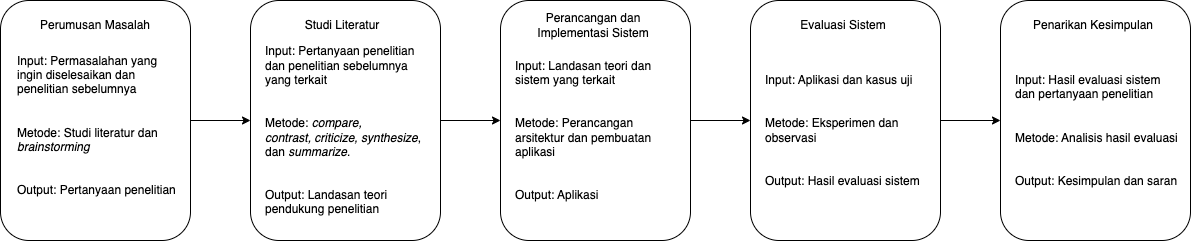
\includegraphics[width=\textwidth]{assets/pics/metode}
	\caption{Langkah penelitian.}
	\label{fig:metode}
\end{figure}

\begin{enumerate}
	\item Perumusan masalah. Penulis merumuskan masalah yang berasal dari permasalahan proses \textit{delivery order} pada sistem Nasional \textit{Single Window} saat ini dan literatur-literatur terkait. Perumusan masalah ini akan menghasilkan pertanyaan penelitian.
	\item Studi literatur. Penulis melakukan pencarian atas penelitian terkait dengan pertanyaan penelitian, dimana penulis melakukan \textit{compare, contrast, criticize, synthesize, dan summarize} atas literatur-literatur terkait sehingga membentuk suatu landasan teori yang dapat menjadi pendukung penelitian.
	\item Perancangan dan implementasi sistem. Dilakukan perancangan arsitektur dan pengembangan sistem aplikasi yang mencakup pengembangan aplikasi web, Hyperledger Fabric SDK, dan jaringan \textit{blockchain} Hyperledger Fabric.
	\item Evaluasi sistem. Akan dilakukan pengujian sistem untuk menjalankan test case untuk proses \textit{Delivery Order} yang diimplementasi menggunakan blockchain.
	\item Penarikan kesimpulan atas hasil evaluasi. Hasil evaluasi akan dikaitkan dengan pertanyaan penelitian yang dirumuskan sebelumnya.

\end{enumerate}


%-----------------------------------------------------------------------------%
\section{Sistematika Penulisan}
\label{sec:sistematikaPenulisan}
%-----------------------------------------------------------------------------%
Sistematika penulisan laporan adalah sebagai berikut:
\begin{itemize}
	\item Bab 1 \babSatu \\
	    Bab ini mencakup latar belakang, cakupan penelitian, dan pendefinisian masalah.
	\item Bab 2 \babDua \\
	    Bab ini mencakup pemaparan terminologi dan teori yang terkait dengan penelitian berdasarkan hasil tinjauan pustaka yang telah digunakan, sekaligus memperlihatkan kaitan teori dengan penelitian.
	\item Bab 3 \babTiga \\
	    Bab ini mencakup metode atau langkah-langkah penelitian yang dilakukan. 
	\item Bab 4 \babEmpat \\
		Bab ini menjelaskan desain aplikasi dan menjelaskan secara rinci implementasi aplikasi yang dibuat.
	\item Bab 5 \babLima \\
	    Bab ini membahas hasil aplikasi yang telah dibuat. Hasil aplikasi akan dikaitkan dengan definisi masalah yang telah dibuat sebelumnya.
	\item Bab 6 \kesimpulan \\
	    Bab ini mencakup kesimpulan akhir penelitian dan saran untuk pengembangan berikutnya.
\end{itemize}

\todo{Anda bisa mengubah atau menambahkan penjelasan singkat mengenai isi masing-masing bab. Setiap tugas akhir pasti ada yang berbeda pada bagian ini.}
